\documentclass[12pt,a4paper,UTF8]{ctexart}
\usepackage{geometry}
\geometry{top=2.5cm,bottom=2.5cm,left=3cm,right=2cm}
\usepackage{setspace}
\setstretch{1.25}
\setlength{\parindent}{2em}
\setlength{\parskip}{0pt}
\usepackage{graphicx}
\usepackage{float}
\usepackage{array}
\usepackage{booktabs}
\usepackage{longtable}
\usepackage{multirow}
\usepackage[table]{xcolor}
\usepackage{hyperref}
\usepackage{enumitem}
\usepackage{pgfplots}
\pgfplotsset{compat=1.18}
\usepackage{titlesec}
\titleformat{\section}{\centering\heiti\zihao{-2}}{\thesection}{0.8em}{}
\titleformat{\subsection}{\heiti\zihao{-3}}{\thesubsection}{0.8em}{}
\titleformat{\subsubsection}{\heiti\zihao{4}}{\thesubsubsection}{0.8em}{}
\hypersetup{hidelinks}
\setlist[itemize]{leftmargin=2em,itemsep=2pt,topsep=2pt}
\setlist[enumerate]{leftmargin=2.2em,itemsep=2pt,topsep=2pt}

\newcommand{\repo}{\texttt{/Users/liuyongze/Documents/AI-agent}}

\begin{document}

\begin{titlepage}
    \thispagestyle{empty}
    \begin{center}
        \vspace*{1.5cm}
        {\heiti\zihao{2} 郑州轻工业大学}\\[0.8cm]
        {\heiti\zihao{2} 软件工程结课报告}\\[2.5cm]
        {\heiti\zihao{-2} AI Agent 系统软件工程结课大作业}\\[0.8cm]
        {\songti\zihao{4} 基于 Spring Boot、React、SSE 与多端协同的智能代理系统工程实践}\\[2.4cm]
        \renewcommand{\arraystretch}{1.8}
        \begin{tabular}{>{\heiti}r p{9cm}}
            题目： & AI Agent 系统的需求、设计、实现与测试全流程分析 \\ 
            院（系）： & 计算机与人工智能学院 \\
            专业班级： & 人工智能 2301 \\
            学生学号： & 542307250114、542307250113、542307250110、542307250112 \\
            学生姓名： & 刘勇泽、刘洋、李容昊、梁家诚 \\
            指导教师： & 夏永泉\quad 支俊 \\
            完成时间： & 2026 年 06 月 \\
        \end{tabular}
        \vfill
        {\songti\zihao{5} 本报告根据《软件工程结课报告》说明书、课程实验一至实验四材料及当前项目仓库实现整理完成。}
    \end{center}
\end{titlepage}

\pagenumbering{Roman}
\tableofcontents
\newpage
\pagenumbering{arabic}

\section{课程任务与报告说明}

\subsection{任务来源与报告定位}
本结课报告以 AI Agent 项目为对象，围绕软件工程课程要求，对项目从立项计划、需求分析、总体设计、详细设计、编码实现、系统测试到综合评价的全过程进行系统整理。报告既保留课程实验一至实验四的阶段性成果，又结合当前仓库的真实代码、接口、测试与运行证据，形成一份完整、可验收、可复盘的工程化文档。

与单一实验报告不同，本报告强调三点：
\begin{enumerate}
    \item 强调全过程视角，不只描述某一实验，而是覆盖“计划-需求-设计-实现-测试-总结”的完整软件生命周期。
    \item 强调工程映射，所有重要结论都尽量能在当前仓库中找到对应的控制器、服务类、数据访问类、前端页面或自动化脚本证据。
    \item 强调量化结果，通过工作量、接口数量、测试数据、代码规模与图表等内容体现项目复杂度和完成度。
\end{enumerate}

\subsection{任务书要求映射}
根据说明书提取，课程结课报告要求采用 A4 幅面、正文规范排版，并由任务书、目录、正文、参考文献和附录等部分组成。为保证交付结果符合课程标准，本文将任务书要求映射到报告结构，如表 \ref{tab:task-mapping} 所示。

\begin{table}[H]
    \centering
    \caption{任务书要求与本报告结构映射}
    \label{tab:task-mapping}
    \begin{tabular}{p{3.2cm}p{8.8cm}}
        \toprule
        任务书要求 & 本报告中的实现方式 \\
        \midrule
        任务书/课题背景明确 & 第 1 章说明课程任务来源、目标及报告定位 \\
        目录完整 & 自动生成目录，覆盖一级到三级标题 \\
        正文包含需求、设计、实现、测试 & 第 2 章至第 7 章分别对应项目计划、需求分析、系统设计、实现映射、测试与综合评价 \\
        参考文献规范 & 第 8 章单独列出参考文献 \\
        附录包含图表与补充材料 & 第 9 章附录收录 UML 图、前端截图、关键类与数据访问说明 \\
        软件工程知识点体现充分 & WBS、角色分工、需求建模、分层架构、数据访问层、测试矩阵、质量评价等内容在正文中逐章展开 \\
        \bottomrule
    \end{tabular}
\end{table}

\subsection{软件工程知识点覆盖说明}
为了严格体现软件工程课程知识点，本报告将项目内容按经典知识体系展开，包括：
\begin{itemize}
    \item 项目计划与 WBS 工作分解结构；
    \item 人员角色划分与职责分配；
    \item 需求获取、需求分析、用例建模与非功能需求定义；
    \item 总体架构设计、模块职责划分、接口设计与数据库设计；
    \item 主要交互功能的实现过程与主要类的内部方法分析；
    \item 数据访问类（Repository/DAO）在持久化层中的职责；
    \item 系统测试、自动化验证、质量评价与综合结论。
\end{itemize}

\section{实验一成果：项目计划与人员分工}

\subsection{项目目标}
AI Agent 项目并不是一个单纯的“聊天页面”，而是一个具有软件工程完整形态的 AI 应用系统。项目目标是构建一套面向 AI + Java 场景的工程化智能代理平台，支持用户认证、会话管理、流式对话、模型路由、工具调用、统计报表以及 Web/CLI 多端协同使用。

从课程角度看，实验一的核心价值在于完成项目立项和计划设计，为后续需求、设计、实现和测试提供边界与节奏约束。项目采用“小组协作 + 分模块负责”的开发方式，确保各成员在软件工程流程中承担明确职责。

\subsection{团队人员分工}
本项目共 4 名成员，采用“组长统筹 + 模块负责人”的协作模式，具体分工如表 \ref{tab:team-division} 所示。

\begin{table}[H]
    \centering
    \caption{项目团队人员分工表}
    \label{tab:team-division}
    \begin{tabular}{p{1.8cm}p{2.5cm}p{7.2cm}}
        \toprule
        成员 & 学号 & 负责内容 \\
        \midrule
        刘勇泽 & 542307250114 & 负责需求分析、系统总体架构、后端核心模块实现、项目统稿与课程验收材料整合。 \\
        刘洋 & 542307250113 & 负责前端页面设计、交互展示、文档排版和运行截图整理。 \\
        李容昊 & 542307250110 & 负责接口联调、脚本验证、CLI 协同、冒烟测试与系统集成验证。 \\
        梁家诚 & 542307250112 & 负责 UML 建模、RAG/Worker 相关方案、部署辅助和性能验证材料整理。 \\
        \bottomrule
    \end{tabular}
\end{table}

该分工符合软件工程中的“职责清晰、边界明确、协作可追踪”原则。尤其是在课程项目中，明确分工可以避免任务重复、责任不清与交付缺口。

\subsection{工作分解结构（WBS）}
根据实验一的项目计划书，项目整体工作可划分为 5 个阶段，如表 \ref{tab:wbs} 所示。

\begin{table}[H]
    \centering
    \caption{项目 WBS 与里程碑安排}
    \label{tab:wbs}
    \begin{tabular}{p{2.3cm}p{2cm}p{2cm}p{6cm}}
        \toprule
        阶段 & 开始时间 & 结束时间 & 主要成果 \\
        \midrule
        需求分析阶段 & 2026-04-15 & 2026-04-18 & 完成需求获取、讨论、分析与确认，输出需求规格说明书。 \\
        原型开发阶段 & 2026-04-19 & 2026-04-23 & 完成交互原型设计、展示和修改确认。 \\
        系统设计阶段 & 2026-04-24 & 2026-04-27 & 完成总体设计、接口设计、详细设计与设计评审。 \\
        系统编码阶段 & 2026-04-28 & 2026-05-10 & 完成后端、前端、CLI 与脚本模块编码和联调。 \\
        系统测试阶段 & 2026-05-11 & 2026-05-16 & 完成功能测试、集成测试、性能测试与测试说明输出。 \\
        \bottomrule
    \end{tabular}
\end{table}

以上 WBS 将抽象的项目目标转化为可执行任务，使每一阶段都具有明确的输入、输出和里程碑，这是典型的软件工程项目计划方法。

\subsection{项目计划中的关键风险}
实验一中已经提前识别了以下关键风险：
\begin{itemize}
    \item 多模型、多工具环境下的接口兼容问题；
    \item SSE 流式推送的稳定性与长连接维护问题；
    \item RAG 检索质量与上下文裁剪对回答效果的影响；
    \item 前后端与 CLI 多端协同带来的联调复杂度；
    \item 部署脚本、环境变量与本地运行条件不一致引发的可重复性问题。
\end{itemize}

这些风险在后续实验二、实验三和实验四中都得到了呼应，说明项目计划不是形式化文档，而是真正约束了项目推进路径。

\section{实验二成果：需求分析与用例建模}

\subsection{需求分析目标}
实验二的目标是形成 AI Agent 系统的需求规格说明书，明确系统建设目标、功能边界、用户角色、业务流程、数据需求与非功能需求，为后续设计和测试奠定需求基线。

\subsection{用户角色与使用场景}
根据实验二文档，系统主要面向两类角色：普通用户与管理员/开发维护人员。其职责如表 \ref{tab:user-roles} 所示。

\begin{table}[H]
    \centering
    \caption{用户角色与职责}
    \label{tab:user-roles}
    \begin{tabular}{p{2.8cm}p{8.2cm}}
        \toprule
        角色 & 职责 \\
        \midrule
        普通用户 & 注册登录系统、创建会话、发送消息、查看历史会话、导出对话记录、使用智能问答与开发陪跑能力。 \\
        管理员/开发维护人员 & 检查系统状态、查看统计与发布报告、执行部署与冒烟验证、维护模型服务和运行环境。 \\
        \bottomrule
    \end{tabular}
\end{table}

\subsection{功能需求分解}
在需求层面，AI Agent 系统主要分为 5 个功能域：
\begin{enumerate}
    \item 用户认证与授权；
    \item 会话管理与消息持久化；
    \item 智能对话与流式输出；
    \item 工具调用、诊断与开发陪跑；
    \item 系统统计、健康检查与报告导出。
\end{enumerate}

这一分解体现了软件工程中的模块化思想，即按职责而非按页面切分系统。

\subsection{需求用例与 UML 支撑}
实验二使用 UML 对系统进行了总体活动图、功能结构图、认证授权用例图、会话管理用例图、多端协同用例图等建模。为了体现需求到设计的连续性，图 \ref{fig:overall-activity} 与图 \ref{fig:function-structure} 分别展示总体活动过程和功能结构。

\begin{figure}[H]
    \centering
    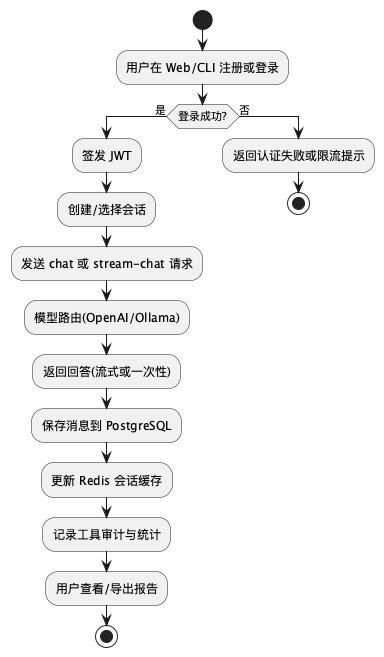
\includegraphics[width=0.86\textwidth]{uml/png/图1_总体活动图.png}
    \caption{AI Agent 系统总体活动图}
    \label{fig:overall-activity}
\end{figure}

\begin{figure}[H]
    \centering
    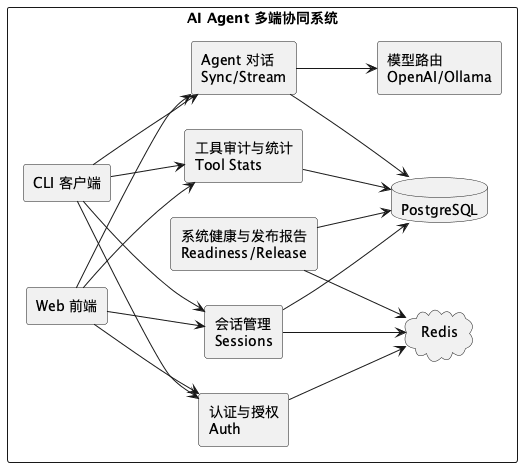
\includegraphics[width=0.86\textwidth]{uml/png/图2_系统功能结构图.png}
    \caption{AI Agent 系统功能结构图}
    \label{fig:function-structure}
\end{figure}

\subsection{非功能需求}
实验二中提出的非功能需求主要包括：
\begin{itemize}
    \item 安全性：采用 JWT 鉴权、密码加密存储、登录限流与路径安全控制；
    \item 性能：普通操作响应不超过 2--3 秒，流式回答要具备首包及时性；
    \item 可维护性：系统采用分层架构和模块化设计，便于后续扩展；
    \item 可部署性：支持 Docker Compose 与脚本化部署；
    \item 可测试性：关键业务流程必须具备明确的测试入口和验证手段。
\end{itemize}

这些非功能需求在实验三设计和实验四测试中均有对应的实现与验证，因此需求基线具有可追踪性。

\section{实验三成果：系统设计与工程实现}

\subsection{总体架构设计}
当前项目采用典型的前后端分离架构，并在此基础上加入 CLI 和桌面端支撑。系统总体架构如图 \ref{fig:architecture} 所示。

\begin{figure}[H]
    \centering
    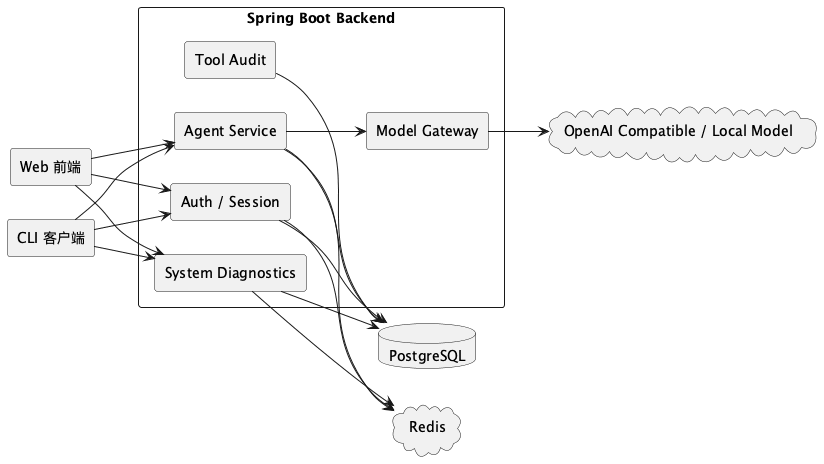
\includegraphics[width=0.92\textwidth]{uml/png/exp3/exp3_01_system_architecture.png}
    \caption{AI Agent 系统总体架构图}
    \label{fig:architecture}
\end{figure}

从分层角度看，系统可划分为：
\begin{itemize}
    \item 表现层：Web 前端、CLI 与 Desktop；
    \item 接口控制层：各类 Controller，负责鉴权、参数校验、接口返回；
    \item 应用服务层：认证、会话、Agent 对话、统计报表与系统诊断；
    \item 基础设施层：数据库、缓存、模型服务、工具执行与外部依赖；
    \item 数据层：PostgreSQL 持久化表与 Redis 运行时缓存。
\end{itemize}

\subsection{数据库设计与数据访问类}
系统数据库使用 PostgreSQL，主要实体包括用户、会话、消息和工具审计记录。与课程要求“数据库使用数据访问类”一致，当前项目并没有在控制器或业务逻辑中直接编写 SQL，而是通过数据访问类（Repository/DAO）封装持久化操作。

\begin{table}[H]
    \centering
    \caption{核心数据访问类与职责}
    \label{tab:data-access}
    \begin{tabular}{p{3.3cm}p{8cm}}
        \toprule
        数据访问类 & 职责说明 \\
        \midrule
        \texttt{UserRepository} & 负责用户账号、密码哈希、令牌版本等用户实体的持久化读写。 \\
        \texttt{ConversationSessionRepository} & 负责会话元数据持久化，包括会话标题、提供商、模型、所属用户等。 \\
        \texttt{MessageRepository} & 负责消息历史的追加、查询与导出所需数据读取。 \\
        \texttt{ToolAuditRepository} & 负责工具调用审计、耗时统计和报表生成所需的原始数据支持。 \\
        \bottomrule
    \end{tabular}
\end{table}

这种设计体现了软件工程中的“数据访问层分离”原则。其优点包括：
\begin{enumerate}
    \item 控制器和业务类不直接依赖底层 SQL 语句；
    \item 持久化逻辑集中，便于维护与测试；
    \item 更容易支撑数据库迁移、性能优化与实体扩展；
    \item 满足实验报告中“数据库设计必须能对应程序结构”的要求。
\end{enumerate}

\subsection{模块设计与职责划分}
为体现设计的可理解性，系统核心模块及主要类职责如表 \ref{tab:modules} 所示。

\begin{table}[H]
    \centering
    \caption{系统核心模块与主要类职责}
    \label{tab:modules}
    \begin{tabular}{p{2cm}p{4.5cm}p{4.8cm}}
        \toprule
        模块 & 主要类/接口 & 职责说明 \\
        \midrule
        认证授权 & \texttt{AuthController}、\texttt{AuthService}、\texttt{JwtService} & 负责注册、登录、刷新令牌、获取当前用户。 \\
        会话管理 & \texttt{SessionController}、\texttt{SessionService} & 负责创建会话、查询历史消息、导出会话数据。 \\
        智能对话 & \texttt{AgentController}、\texttt{AgentService}、\texttt{ModelGateway} & 负责同步/流式对话、模型路由与 Agent 执行循环。 \\
        工具编排 & \texttt{AgentToolOrchestrator}、\texttt{CodeToolService} & 负责搜索代码、读取文件、分析 POM、执行工具并返回结果。 \\
        统计报表 & \texttt{ToolStatsController}、\texttt{ReleaseReportController} & 负责工具统计、健康报告和发布报告导出。 \\
        系统诊断 & \texttt{SystemController}、\texttt{SystemDiagnosticsService} & 负责健康检查、模型列表与依赖可用性验证。 \\
        \bottomrule
    \end{tabular}
\end{table}

\subsection{主要交互功能的具体实现过程}
按照你的要求，本文选择“基于 SSE 的流式对话”作为主要交互功能进行具体实现过程分析。该功能既是系统最核心的用户价值点，也是软件工程上最能体现接口设计、状态管理、线程控制和异常处理的模块。

\subsubsection{流式对话交互过程说明}
从用户角度看，流程是“输入问题 $\rightarrow$ 发送请求 $\rightarrow$ 实时接收回答 $\rightarrow$ 保存会话历史”；从程序实现角度看，完整流程如图 \ref{fig:chat-sequence} 所示。

\begin{figure}[H]
    \centering
    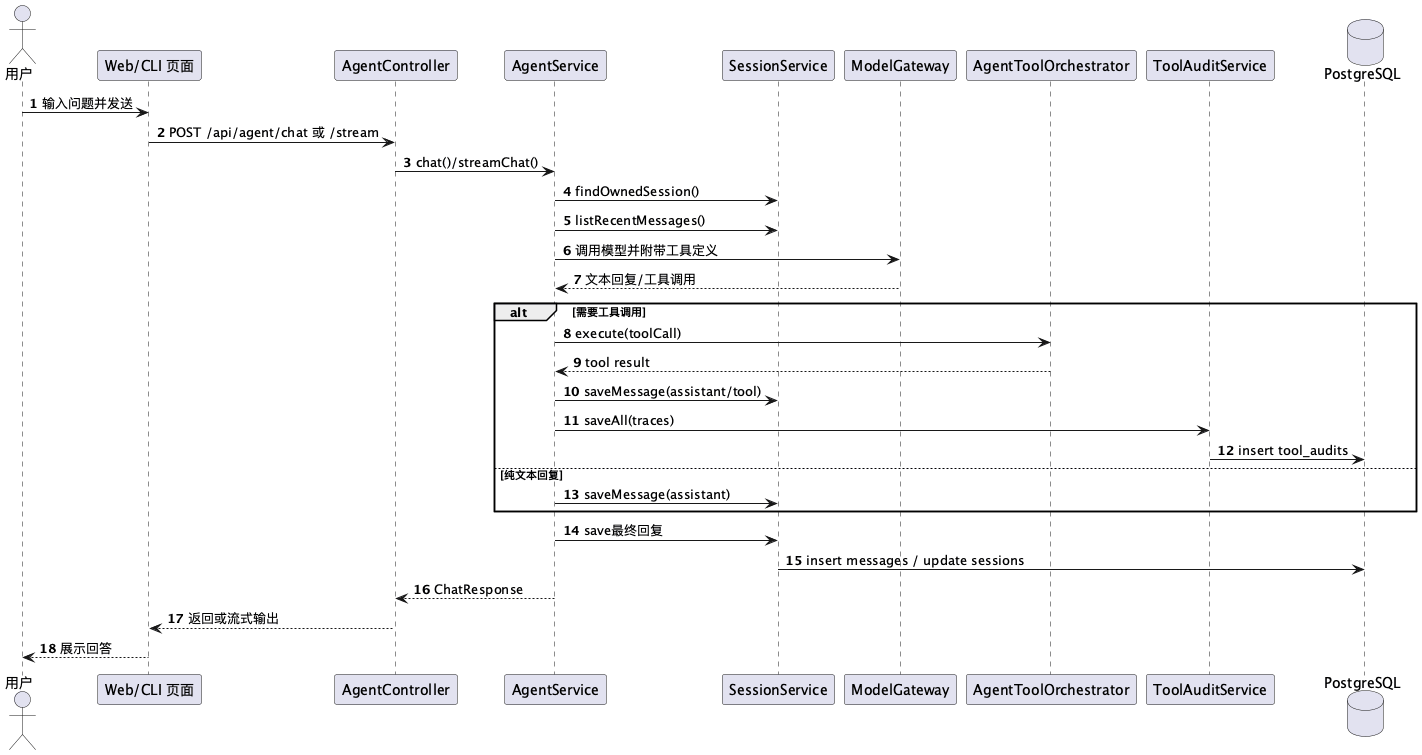
\includegraphics[width=0.88\textwidth]{uml/png/exp3/exp3_06_chat_flow_sequence.png}
    \caption{流式对话实现过程时序图}
    \label{fig:chat-sequence}
\end{figure}

其具体实现过程可细化为 8 个步骤：
\begin{enumerate}
    \item 前端或 CLI 调用 \texttt{POST /api/v1/agent/chat/stream}，提交 \texttt{sessionId}、消息内容及可选模型参数。
    \item \texttt{AgentController} 首先完成用户身份校验和频率限制检查，然后创建 SSE 响应通道。
    \item \texttt{SessionService} 验证该会话是否属于当前用户，并将用户消息先持久化到数据库。
    \item \texttt{ModelRoutingService} 根据请求参数、会话配置和默认配置解析当前实际使用的模型提供商与模型名称。
    \item \texttt{AgentService.buildMessages(...)} 负责将系统提示词、历史消息、上下文预算和工具定义拼装成模型输入。
    \item \texttt{AgentService.executeLoop(...)} 驱动 Agent 循环：如果模型返回普通文本，则以 \texttt{chunk} 事件持续推送；如果模型返回工具调用请求，则交由 \texttt{AgentToolOrchestrator} 执行，再把工具结果回填到上下文中继续推理。
    \item 在流式过程中，服务端按固定时间间隔发送 \texttt{heartbeat} 事件，防止长连接在网络中间设备上被过早关闭。
    \item 对话完成后，\texttt{persistFinalAssistant(...)} 将最终回复和工具轨迹保存入库，供历史消息查询、报表统计和后续导出使用。
\end{enumerate}

这一实现过程体现了多个软件工程知识点：接口设计、服务分层、状态保持、异常恢复、资源管理和日志可追踪性。

\subsection{针对主要类描述其内部方法}
按照课程要求，本文选择系统中最核心的业务类 \texttt{AgentService} 进行内部方法分析。该类是 AI Agent 系统的应用编排中枢，负责把会话、模型、工具、上下文和持久化连接成一个完整闭环。

\begin{table}[H]
    \centering
    \caption{AgentService 主要内部方法说明}
    \label{tab:agentservice}
    \begin{tabular}{p{4.2cm}p{7.2cm}}
        \toprule
        方法 & 作用说明 \\
        \midrule
        \texttt{chat(UUID, ChatRequest)} & 同步对话入口，负责会话校验、模型解析、用户消息持久化并返回完整回答。 \\
        \texttt{streamChat(UUID, ChatRequest, ...)} & 流式对话入口，负责发送元数据、输出文本分块、维护心跳和结束状态。 \\
        \texttt{executeLoop(...)} & Agent 核心执行循环，轮询模型文本响应和工具调用结果，并决定是否继续迭代。 \\
        \texttt{buildMessages(...)} & 根据系统提示词、历史消息、工具定义和 RAG 信息拼装模型输入。 \\
        \texttt{sliceByTokenBudget(...)} & 按 token 预算裁剪历史上下文，避免请求输入过长。 \\
        \texttt{sanitizeSystemContext(...)} & 对动态上下文中的敏感信息进行清洗和截断。 \\
        \texttt{resolveContextTokenBudget(...)} & 解析当前对话实际使用的上下文长度限制。 \\
        \texttt{persistFinalAssistant(...)} & 将最终回复与工具轨迹持久化，为消息导出与统计报表提供数据基础。 \\
        \bottomrule
    \end{tabular}
\end{table}

从设计角度看，\texttt{AgentService} 的方法划分较好地体现了“高内聚、低耦合”的原则：对外只暴露同步和流式两个用例入口，对内则把上下文组装、预算裁剪、工具循环、结果持久化等细节拆解为独立方法，便于维护和测试。

\section{实现结果与量化数据分析}

\subsection{仓库实现规模数据}
为了体现结课项目不是“纸面设计”，本文对当前仓库的主要代码模块做了静态规模统计，结果如表 \ref{tab:loc} 所示。

\begin{table}[H]
    \centering
    \caption{当前仓库代码规模统计}
    \label{tab:loc}
    \begin{tabular}{p{2.2cm}p{2.2cm}p{2.2cm}}
        \toprule
        模块 & 文件数 & 代码行数 \\
        \midrule
        后端主代码 & 116 & 6711 \\
        后端测试代码 & 21 & 1823 \\
        Web 前端 & 39 & 4086 \\
        CLI 客户端 & 10 & 1634 \\
        Desktop 端 & 4 & 562 \\
        \bottomrule
    \end{tabular}
\end{table}

\begin{figure}[H]
    \centering
    \begin{tikzpicture}
        \begin{axis}[
            width=0.9\textwidth,
            height=7cm,
            ybar,
            symbolic x coords={后端,后端测试,Web,CLI,Desktop},
            xtick=data,
            ylabel={代码行数},
            ymin=0,
            nodes near coords,
            bar width=18pt,
            enlarge x limits=0.15,
            ymajorgrids=true,
            grid style=dashed,
        ]
        \addplot[fill=blue!55] coordinates {
            (后端,6711)
            (后端测试,1823)
            (Web,4086)
            (CLI,1634)
            (Desktop,562)
        };
        \end{axis}
    \end{tikzpicture}
    \caption{项目代码规模图}
    \label{fig:loc-chart}
\end{figure}

\subsection{接口规模与控制器分布}
当前主分支为 \texttt{main}，最近提交短哈希为 \texttt{570206c}。对后端控制器统计后，共有 24 个核心 REST 接口，分布如表 \ref{tab:endpoints} 所示。

\begin{table}[H]
    \centering
    \caption{控制器接口数量分布}
    \label{tab:endpoints}
    \begin{tabular}{p{3.2cm}p{2.5cm}}
        \toprule
        控制器 & 接口数量 \\
        \midrule
        AgentController & 3 \\
        AuthController & 5 \\
        CoachController & 5 \\
        SessionController & 5 \\
        ReleaseReportController & 2 \\
        SystemController & 2 \\
        ToolStatsController & 2 \\
        合计 & 24 \\
        \bottomrule
    \end{tabular}
\end{table}

\begin{figure}[H]
    \centering
    \begin{tikzpicture}
        \begin{axis}[
            width=0.9\textwidth,
            height=7cm,
            ybar,
            symbolic x coords={Agent,Auth,Coach,Session,Release,System,ToolStats},
            xtick=data,
            ylabel={接口数量},
            ymin=0,
            ymax=6,
            nodes near coords,
            bar width=15pt,
            enlarge x limits=0.12,
            ymajorgrids=true,
            grid style=dashed,
            x tick label style={rotate=20,anchor=east}
        ]
        \addplot[fill=teal!60] coordinates {
            (Agent,3)
            (Auth,5)
            (Coach,5)
            (Session,5)
            (Release,2)
            (System,2)
            (ToolStats,2)
        };
        \end{axis}
    \end{tikzpicture}
    \caption{控制器接口数量柱状图}
    \label{fig:endpoint-chart}
\end{figure}

\subsection{前端与多端运行界面}
为了体现项目具备可运行的真实界面，而不是只停留在文字设计层，图 \ref{fig:frontend-auth}、图 \ref{fig:frontend-chat} 和图 \ref{fig:frontend-stats} 给出了当前系统的典型运行截图。

\begin{figure}[H]
    \centering
    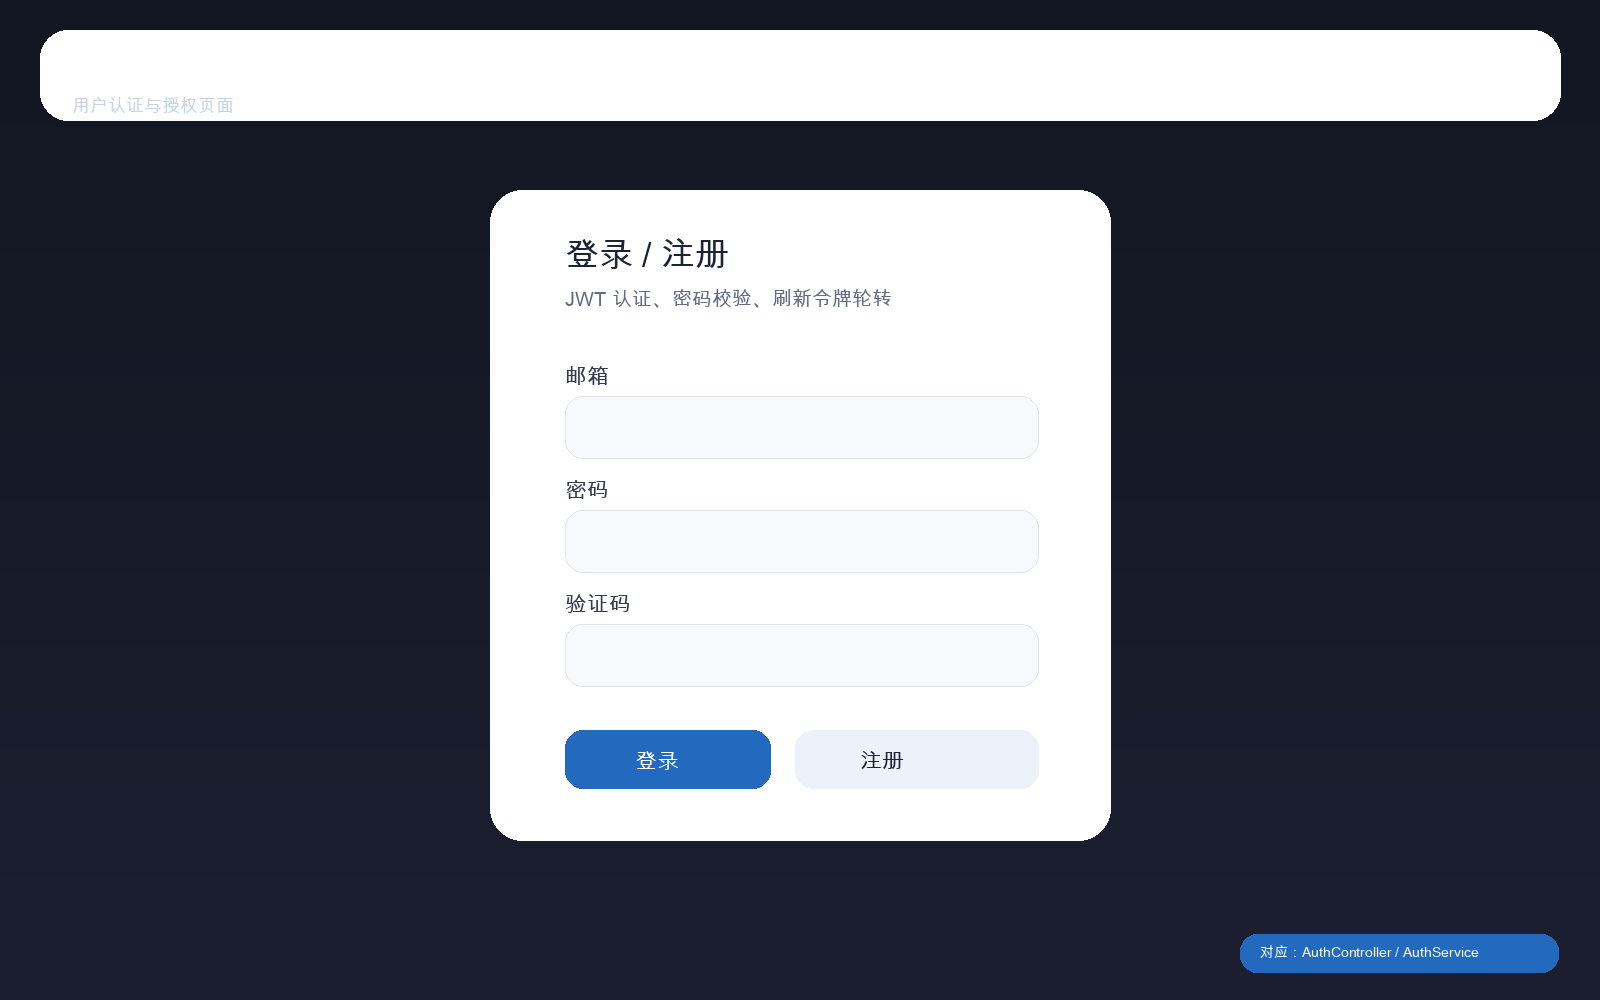
\includegraphics[width=0.85\textwidth]{artifacts/exp3/frontend/exp3_frontend_auth.png}
    \caption{系统认证页面截图}
    \label{fig:frontend-auth}
\end{figure}

\begin{figure}[H]
    \centering
    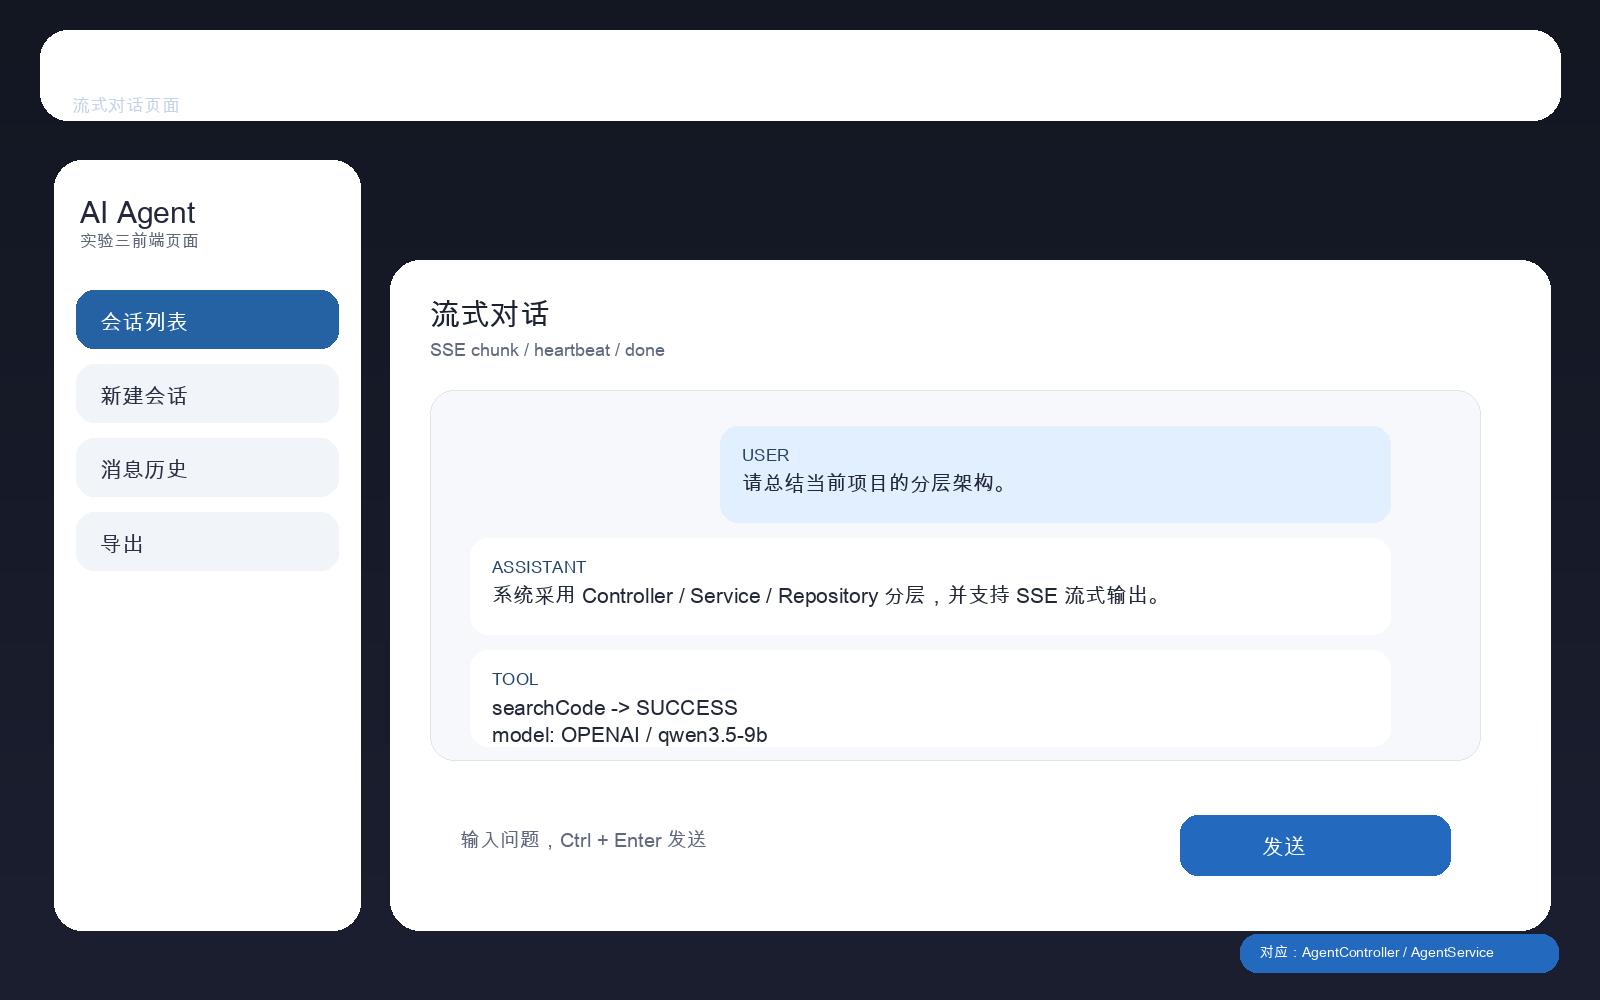
\includegraphics[width=0.85\textwidth]{artifacts/exp3/frontend/exp3_frontend_chat.png}
    \caption{系统聊天页面截图}
    \label{fig:frontend-chat}
\end{figure}

\begin{figure}[H]
    \centering
    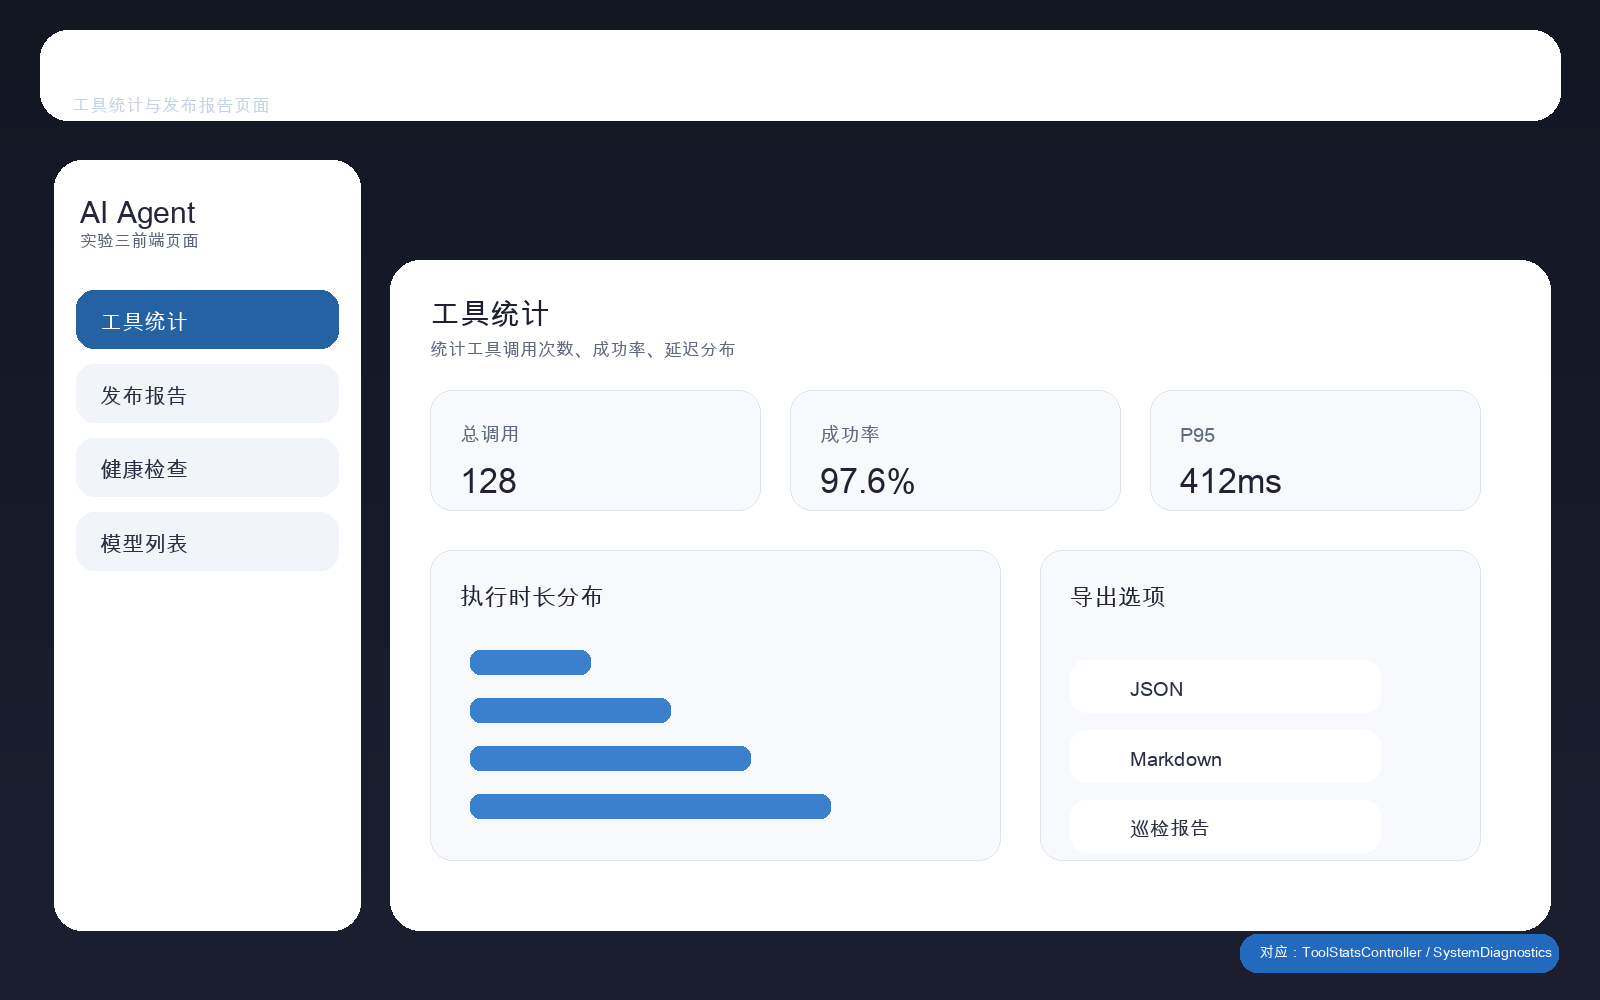
\includegraphics[width=0.85\textwidth]{artifacts/exp3/frontend/exp3_frontend_stats.png}
    \caption{系统统计与诊断页面截图}
    \label{fig:frontend-stats}
\end{figure}

\section{实验四成果：系统测试与质量评价}

\subsection{测试角色与工作量}
实验四并不是简单“跑几个接口”，而是围绕黑盒、白盒、集成、并发与协同测试展开。根据实验四文档，团队测试总预算工时为 56 人时，个人投入分布如图 \ref{fig:hours-chart} 所示。

\begin{figure}[H]
    \centering
    \begin{tikzpicture}
        \begin{axis}[
            width=0.82\textwidth,
            height=6.5cm,
            ybar,
            symbolic x coords={刘勇泽,刘洋,李容昊,梁家诚},
            xtick=data,
            ylabel={工时/h},
            ymin=0,
            ymax=18,
            nodes near coords,
            bar width=20pt,
            enlarge x limits=0.2,
            ymajorgrids=true,
            grid style=dashed,
        ]
        \addplot[fill=green!55!black] coordinates {
            (刘勇泽,16)
            (刘洋,12)
            (李容昊,14)
            (梁家诚,14)
        };
        \end{axis}
    \end{tikzpicture}
    \caption{测试工作量分配图}
    \label{fig:hours-chart}
\end{figure}

\subsection{核心测试用例设计}
根据实验四，系统测试围绕 6 个核心测试用例展开，如表 \ref{tab:testcases} 所示。

\begin{table}[H]
    \centering
    \caption{核心测试用例矩阵}
    \label{tab:testcases}
    \begin{tabular}{p{2.8cm}p{2.4cm}p{1.6cm}p{4cm}}
        \toprule
        编号 & 测试主题 & 类型 & 覆盖重点 \\
        \midrule
        TestCase-FUNC-01 & 会员注册表单边界测试 & 黑盒 & 覆盖非法邮箱、重复注册、空白密码等情况。 \\
        TestCase-FUNC-02 & JWT 安全拦截与登录限流 & 白盒+接口 & 覆盖缺失 Token、伪造签名、过期 Token、频率超限。 \\
        TestCase-FUNC-03 & 会话生命周期与导出 & 集成 & 覆盖会话创建、消息持久化、JSON/Markdown 导出。 \\
        TestCase-FUNC-04 & SSE 流式对话与模型降级 & 集成 & 覆盖分块、心跳、模型异常与本地 Mock 兜底。 \\
        TestCase-FUNC-05 & 健康检查与统计报表 & 接口+系统 & 覆盖 readiness、tool stats、release report。 \\
        TestCase-FUNC-06 & Web/CLI 协同与高并发负载 & 性能+协同 & 覆盖双端一致性及 50--100 用户压测。 \\
        \bottomrule
    \end{tabular}
\end{table}

\subsection{当前自动化验证数据}
对当前仓库的测试结果进行统计后，得到以下自动化验证数据：
\begin{itemize}
    \item 后端 surefire 共统计 47 个测试；
    \item 其中通过 36 个，跳过 11 个；
    \item 跳过项主要是依赖 Docker/Testcontainers 的集成测试；
    \item 这些测试集中覆盖认证、Agent 流程、启动校验、工具统计和发布报告等关键模块。
\end{itemize}

\begin{table}[H]
    \centering
    \caption{自动化测试结果汇总}
    \label{tab:test-summary}
    \begin{tabular}{p{3.2cm}p{2.4cm}}
        \toprule
        指标 & 数值 \\
        \midrule
        总测试数 & 47 \\
        通过数 & 36 \\
        跳过数 & 11 \\
        通过率（按已执行） & 100\% \\
        跳过原因 & 依赖 Docker/Testcontainers 的集成环境 \\
        \bottomrule
    \end{tabular}
\end{table}

\subsection{质量评价}
结合实验四测试记录与当前仓库实现，可以得出以下质量评价：
\begin{enumerate}
    \item 功能完整性较高。认证、会话、流式对话、统计报表和开发陪跑模块均已具备真实实现。
    \item 分层结构清晰。控制器、服务类、数据访问类、模型适配层和工具执行层边界明确。
    \item 工程化程度较好。项目具备 README、脚本、测试、UML 图、前端截图和实验文档多类证据。
    \item 仍有进一步提升空间。前端自动化测试规模、完整集成环境覆盖和更细粒度的性能压测仍可继续增强。
\end{enumerate}

\section{综合结论}
从软件工程全过程视角分析，AI Agent 项目已经形成“计划-需求-设计-实现-测试-验证”的完整闭环：
\begin{itemize}
    \item 实验一完成了项目计划、里程碑和人员分工；
    \item 实验二完成了需求基线、角色分析和功能建模；
    \item 实验三完成了分层架构、模块设计、主要交互流程和类方法设计；
    \item 实验四完成了系统级测试、质量评价和可量化验证；
    \item 当前仓库则提供了真实代码、接口、图表、截图和测试证据。
\end{itemize}

因此，本项目已经不再是一个单点功能 Demo，而是一份具备课程要求、工程结构、实现深度和验收证据的软件工程结课项目。

\section{参考文献}
\begin{enumerate}
    \item 《软件工程结课报告》说明书，郑州轻工业大学课程资料。
    \item 《AI Agent 系统》项目计划书，课程实验一成果材料。
    \item 《AI Agent 系统》需求规格说明书，课程实验二成果材料。
    \item 《AI Agent 系统》设计规格说明书，课程实验三成果材料。
    \item 《AI Agent 系统》软件测试说明书，课程实验四成果材料。
    \item \repo\ 中的 \texttt{README.md}、\texttt{Code\_Wiki.md}、后端源码、前端源码及测试代码。
    \item Spring Boot、React、PostgreSQL、Redis、Server-Sent Events 相关官方文档。
\end{enumerate}

\section{附录}

\subsection{附录 A：关键 UML 图补充}
\begin{figure}[H]
    \centering
    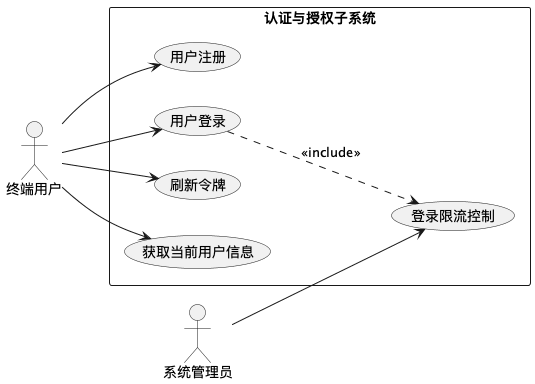
\includegraphics[width=0.84\textwidth]{uml/png/图3_认证与授权用例图.png}
    \caption{认证与授权用例图}
\end{figure}

\begin{figure}[H]
    \centering
    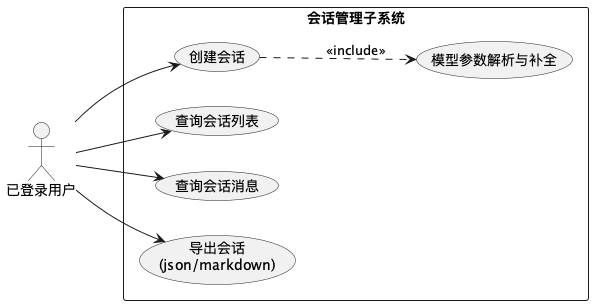
\includegraphics[width=0.84\textwidth]{uml/png/图4_会话管理用例图.png}
    \caption{会话管理用例图}
\end{figure}

\begin{figure}[H]
    \centering
    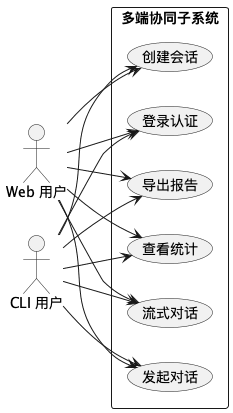
\includegraphics[width=0.84\textwidth]{uml/png/图7_Web与CLI多端协同用例图.png}
    \caption{Web 与 CLI 多端协同用例图}
\end{figure}

\subsection{附录 B：报告使用的核心事实数据}
\begin{itemize}
    \item Git 分支：\texttt{main}
    \item 最近提交：\texttt{570206c}
    \item 后端控制器接口总数：24
    \item 后端测试总数：47
    \item 当前代码规模：后端 6711 行，前端 4086 行，CLI 1634 行
\end{itemize}

\end{document}
